\documentclass[a4paper]{article}

\usepackage[english]{babel}
\usepackage[utf8x]{inputenc}
\usepackage{graphicx}
\usepackage[ELEC]{aaltologo}
\usepackage{verbatim}
\usepackage[bf,small]{caption}

\begin{document}
% Titlepage
\begin{titlepage}

% Upper part of the page
\begin{flushleft}
\AaltoLogoSmall{1}{?}{aaltoYellow} \\
Department of Communications and Networking \\
S-38.3159 Protocol Design P \\
Spring 2014
\end{flushleft}

\vspace{8cm}
% Title
\begin{center}
  {\LARGE \textbf{aNSA is Not a Sensor Aggregator}}\\
  {\LARGE Protocol specification}
\end{center}

\vfill

\begin{center}
\begin{tabular}{rll}
	Student 1:	& Riku Lääkkölä 	& 69896S \\
				& riku.laakkola@aalto.fi & \\    
    Student 2: 	& Tero Marttila		& 78949E \\
    			& tero.marttila@aalto.fi & \\
    Student 3:	& Tero Paloheimo	& 78510C \\
    			& tero.paloheimo@aalto.fi & \\
\end{tabular}
\end{center}

\end{titlepage}

\tableofcontents
\newpage

\section{Introduction}
This document describes a UDP-based protocol for use in a client-server based publish-subscribe model.
The server receives sensor updates, and publishes the sensor values to subscribed clients.
Individual clients may query for the list of available sensors, and update their set of subscribed sensors.
The server will monitor sensor availability, and update the client when sensors become available or unavailable.
The protocol is designed for real-time purposes, and as such, provides ordered unreliable transmission, periodically transmitting the newest state.

The bidirectional control streams are identified by a type code and separate sequence counters for client and server transmissions, which are acknowledged by the recipient.
The subscription protocol is based on the use of soft state, with the client and server transmitting their full subscription state on each change.
It is expected that the amount of subscription-related traffic will remain minor compared to the actual \textbf{publish}-traffic.

The unidirectional data stream is used by the server to publish the most recent sensor values to the client.
The client will periodically acknowledge the received sensor publishes, which is used by the server as a feedback channel for keepalive and congestion control purposes.
It is vitally important for the server to handle clients that disappear, timing out their subscriptions.

The messages are transmitted as UDP packets between the client and server, using a fixed port on the server, and an arbitrary port on the client.
All messages are transmitted and received using the same pair of \- addresses/ports.
If the client changes to a different address, it must create a new subscription to the server, and the previous one will time out.

\section{Message format}
The protocol is based on a hybrid binary/text encoding, using a fixed-size binary header for transport control purposes, and a JSON-encoded variable-length payload.
The message header format is described in Figure \ref{fig:header}. The header
is transmitted in network byte order, that is, big-endian byte order. The 
Magic-field is an identifier for our protocol and also works as a version
number. The Type-field denotes the message type (subscribe, unsubscribe, etc.),
the flags are described in Table \ref{tbl:header_values}. The remaining bits are 
reserved for future use. The following fields are for sequence numbers: 
\textbf{Ack-Seq} is used for acknowledging receiver sequence numbers, and 
\textbf{Seq} is used for the sender sequence number. The sender sequence number
should start from an arbitrary value that must not be zero, and must wrap around to $1$. Sequence number comparisons should behave cyclically mod $2^{31}$, i.e. $2^{31} > 1 > 2^{32} - 1 > 2^{31} + 1$.

\begin{figure}
	\begin{center}
		\verbatiminput{headerfmt.txt}
		\caption{Message format}
		\label{fig:header}
	\end{center}
\end{figure}

The range of possible messages and associated header field values are listed in Table 
\ref{tbl:messages}.

\begin{table}
\begin{center}
\caption{Message types. The header field values are shown in Table \ref{tbl:header_values}.}
\begin{tabular}{|l|l|l|l|l|l|l|}
\hline
						& 							& \multicolumn{4}{c|}{Header field value} &	\\
Message					& Direction 				& N	& T	& Ack-seq				& Seq	&	Payload \\
\hline
subscribe-query			& Cl $\rightharpoonup$ S		& 1	& 0 	& 0						& 0	&	\\
\hline
subscribe-queryresponse	& Cl $\leftharpoondown$ S	& 1	& 0		& 0						& 0	&	x \\
\hline
subscribe-request		& Cl $\rightharpoonup$ S		& 1	& 0		& 0						& \emph{Cl-sseq++} &
	x \\
\hline
subscribe-response		& Cl $\leftharpoondown$ S	& 1	& 0		& \emph{Cl-sseq}	& \emph{S-sseq++} &	
	x \\
\hline
subscribe-update		& Cl $\leftharpoonup$ S		& 1	& 0		& 0						& \emph{S-sseq++} &
	x \\
\hline
subscribe-ack			& Cl $\rightharpoondown$ S	& 1	& 0		& \emph{S-sseq}	& 0	&	\\
\hline
publish					& Cl $\leftharpoonup$ S		& 1	& 1		& 0						& \emph{S-pseq++} &
	x \\
\hline
publish	(/w NoAck)      & Cl $\leftharpoonup$ S		& 0	& 1		& 0						& \emph{S-pseq++} &
	x \\
\hline
publish-ack				& Cl $\rightharpoondown$ S	& 1	& 1		& \emph{S-pseq}			& \emph{nrecvd}	&	\\
\hline
teardown		      & Cl $\rightharpoonup$ S		& 1	& 2		& 0			& 0	& \\
\hline
teardown-ack		& Cl $\leftharpoondown$ S 		& 1 & 2		& 0			& 0 &	\\
			
\hline
\end{tabular}
\label{tbl:messages}
\end{center}
\end{table}

\begin{table}
\caption{The header field values.}
\begin{description}
  \item[Magic] This field has value \texttt{0x43} for protocol version 2
  \item[N] 	The non-acknowledgement (``NoAck'') flag (only used for \textbf{publish}) being set indicates that
  			the ack message that would normally be sent in response to a nonzero seq should be supressed.
  \item[C] 	The compression flag being set means that the payload has been compressed using the
  			\texttt{zlib} DEFLATE format.
  \item[T/Type] Message type field
  \item[Cl] Client
  \item[S] Server
  \item[sseq] Subscribe message specific sequence number
  \item[pseq] Publish message specific sequence number
  \item[nrecvd] Number of publishes received by the client so far
\end{description}
\label{tbl:header_values}
\end{table}

\pagebreak

Below is a list of the various messages and their semantics. The payloads of the
messages are defined in Section \ref{payload-format}.
\begin{description}
	\item[subscribe-query] Client initiated query of the available 
	sensors. The server sends the sensor list and the client processes it.
    
	\item[subscribe-queryresponse] Response from the server to 
	\emph{subscribe-query}, contains a list of available sensor names. 
    
	\item[subscribe-request] A message sent by the client to update its sensor
	subscription. Contains a list of the sensors to which the client wants to
	subscribe. This message must be acknowledged by the server. If the client
    wants to subscribe to one or more sensors, the payload must be a list with
    the sensor names. The client may subscribe to all sensors. Unsubscribing,
    that is, subscribing to no sensors is done by sending an empty list.

	\item[subscribe-response] Server acknowledgement to the 
	\emph{subsribe-request} message. The message contains a dictionary which
    contains all the sensors and separately specifies the subscribed sensors.
    The subscribed sensors have a truthy value and the unsubscribed have a falsey
    value. 

  	After receiving the \emph{subscribe-request} message, the server will
    respond with an falsey \emph{subscribe-response} message, which the client
    will acknowledge. Only after receiving this acknowledgement message,
    will the server send the ``real'' acknowledgement with the subscribed sensors.
    This three-way handshake is done to prevent using the subscribe procedure
    for DDoS amplification attacks.

	\item[subscribe-update] A message from the server containing an updated
	list of sensors. This message is sent whenever the sensors are updated,
	that is, a sensor is added or removed. This message needs to be acknowledged 
	by the client and is sent until an acknowledgement is received. The payload
    must have the same format as the \emph{subscribe-response} message.
    
	\item[subscribe-ack] Client initiated message which acknowledges the 
	\emph{subscribe-update} message.
    
	\item[publish] The server-initiated message contains the values of
	the subscribed sensors. If this message is lost, it is not retransmitted but
	new values are sent instead. The payload is a list with the sensor values 
    (dictionary) from each sensor.
    
	\item[publish (/w NoAck unset)] Like the ``normal'' \emph{publish} message
	but this must be acknowledged by the client. The acknowledgement is used
	by the server to check whether the other party is still	available, and measure
    congestion. This message has the same payload format as the unacknowledged
    \emph{publish} message.
    
	\item[publish-ack] Message from the client which acknowledges the previous
	\emph{publish (/w NoAck unset)} message.
    
	\item[teardown] A message sent by the client indicating that is 
	wants to end the communication with the server. This message must be 
	acknowledged by the server. A client sends this message until it receives 
	the \emph{teardown-ack} message as an acknowledgement. If the server 
	receives this message from an unknown client, it will respond with a
	\emph{teardown-ack} message.
    
	\item[teardown-ack] Server response to the \emph{teardown} message
	sent by a client. After sending this message, the server timeouts for $T_t$
    seconds, and if no retransmits of \emph{teardown} arrive, the connection is
    terminated and resources are freed.
\end{description}

The \emph{subscribe-*} messages have a timer mechanism.
When a message is sent with an incremented sequence number, the timer is set.
Receiving a message with the matching \emph{type} and \emph{ack-seq} field will 
clear the timer. If the timer expires after $T$ seconds, where $T$ is at most
ten seconds but may be smaller, the previously sent message will be retransmitted (using the same seq).
Handling of received messages is based on the \emph{seq} field.
The highest received \emph{seq} is recorded, acked and processed.
A duplicate \emph{seq} corresponding to the updated seq is considered a duplicate, and is acked without being processed.
A lower \emph{seq} than recorded indicates packet reordering and is dropped.

\section{Protocol description}


\subsection{Subscribing and unsubscribing}
The protocol supports an optional \emph{subscribe-query}/\emph{subscribe-queryresponse} handshake which the client can use to prepare its subscription list.
The client sends a \emph{subscribe-query} message to the server.
The server will then reply with a \emph{subscribe-queryresponse} message, which contains the list of currently available sensors.

Setting up the subscription session uses a \emph{subscribe-request}/\emph{subscribe-request}/\emph{subscribe-ack}/\emph{subscribe-update} handshake sequence.
The client initiates the session by sending a \emph{subscribe-request} message, which contains a list of sensors to which the client wants to subscribe.
The server will then initially respond with a \emph{subscribe-response} message with an empty payload.
The client completes the three-way handshake using an \emph{subscribe-ack} message, which initiates the session.
The server immediately sends the initial \emph{subscribe-update} message containing the new subscription state, and starts sending \texttt{publish} messages if appropriate.

A normal sequence of message sent when a client subscribes to some sensors is shown in Figure \ref{fig:sub_normal}.
The same sequence with lost packets is shown in Figure \ref{fig:sub_lost}.

\begin{figure}[htb]
	\centering
    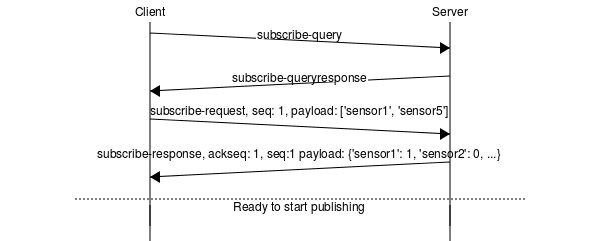
\includegraphics[width=\textwidth]{figures/subscribe_normal.pdf}
    \caption{A normal subscription sequence.}
    \label{fig:sub_normal}
\end{figure}

\begin{figure}[htb]
	\centering
    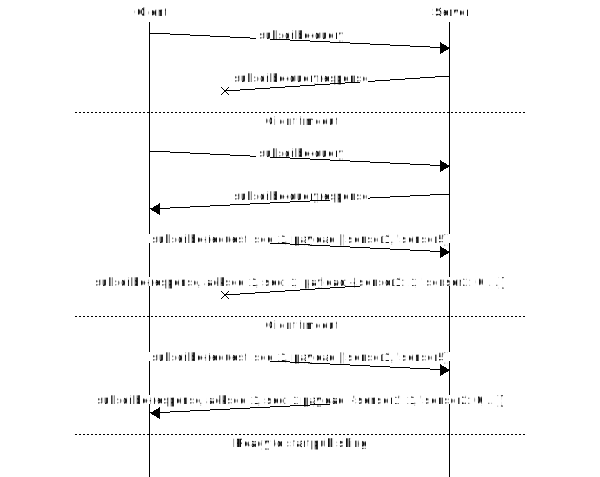
\includegraphics[width=\textwidth]{figures/subscribe_lost.pdf}
    \caption{A subscription sequence with packet loss.}
    \label{fig:sub_lost}
\end{figure}

The client may update its subscription set at any point by sending a new \emph{subscribe-request} message with a new sensor list, which may contain any arbitrary subset or superset of the previous subscription sensor set, including an empty set to unsubscribe from all sensors.
The server will acknowledge the updated subscription by sending a new \emph{subscribe-response} message with the new subscription state.

When the available sensors change, the server will send a new list of subscribed sensors to the clients with the \emph{subscribe-update} message.
The client will acknowledge the reception by sending the \emph{subscribe-ack} message.

A client terminates the connection by sending the \emph{teardown} message to the server.
It expects a response from the server and will retransmit the teardown until a response is received.
The server acknowledges the reception of the the message by sending a sending a\emph{teardown-ack} message and immediately releasing any resources allocated to the client session.
If the server receives a \emph{teardown} from a client that has no resources currently allocated for it, the server must respond with a matching \emph{teardown-ack}.

\subsection{Publish}
Whenever a new sensor value is received at the server it will be sent to the 
clients who are subscribed to the selected sensor. The updates are sent with
the \emph{publish} message, which contains the current value of the sensor.
These messages are not retransmitted and generally not acknowledged, except in the case of the on/off -type). Publish
messages with the ``NoAck'' bit unset are sent every $T_s$ seconds even if there
is no sensor data to publish. The payload of these messages are last states
of the subscribed on/off sensors. These messages must be acknowledged by the client 
with the \emph{publish-ack} message, but the server may continue sending normal 
\emph{publish} messages without waiting for the ack to arrive. A publish message
sequence is shown in Figure \ref{fig:pub_normal}.

\begin{figure}
	\centering
    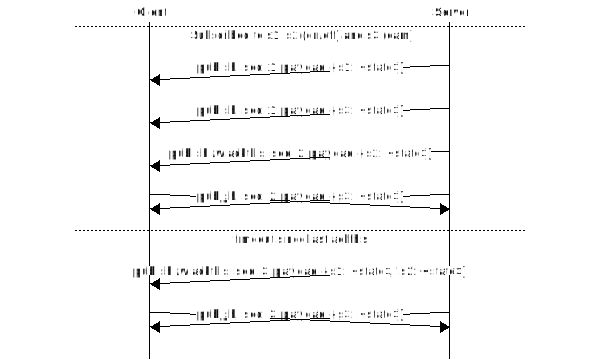
\includegraphics[width=\textwidth]{figures/publish_normal.pdf}
    \caption{A publish message sequence.}
    \label{fig:pub_normal}
\end{figure}

The purpose of these messages is to act as a ``keepalive'' mechanism (and also double
as a reliability mechanism for the on/off sensors). If acknowledgements from a client
are not received within a time of $N \cdot T_s$ seconds for some value of $N$, the 
server will timeout the client. The same mechanism also works in the opposite 
direction, if publish messages are not received from the server within 
$M \cdot T_s$ seconds for some value of $M$,
the server is considered to be unavailable and the client will time out. The 
$T_s$ timeout must be ten seconds and $M \geq 3, N \geq 3$. The time it takes for an acknowledgement to be received after the sending of
a publish message may be used to estimate the RTT.
The \emph{publish-ack} message sent by the client includes both the number of messages sent by the server (\emph{ack-seq}) as well as the number of publish messages received by the client (\emph{seq}).
The server may use this information to determine packet loss for congestion control purposes.

\subsection{Payload format}
\label{payload-format}

The message payload is a JSON-formatted object.

The JSON values \texttt{false}, \texttt{0}, \texttt{[]} and \texttt{\{\}} are defined to evaluate to boolean false.

\subsubsection{\emph{subscribe-request}}
The \emph{subsribe-request} message contains either a boolean value, a list of sensor names, or a dict of sensor names and complex aggregation subscriptions.

To subscribe to all available sensors (including sensors becoming available in the future), the client may send a subscribe message containing a boolean:
\begin{verbatim}
true
\end{verbatim}

To subscribe to a set of sensors with non-aggregated publishes, the client may send a subscribe message containing:
\begin{verbatim}
[ 'temp:1', 'device:1' ]
\end{verbatim}

To subscribe to a set of sensors with complex aggregation rules, the client may send a subscribe message containing an aggregation expression dict:
\begin{verbatim}
{ 'device:1': true, 'temp:1': { ... } }
\end{verbatim}

To unsubscribe from all sensors (while keeping the session open), the client may send a boolean false:
\begin{verbatim}
false
\end{verbatim}

\subsubsection{\emph{subscribe-response}}
The \emph{subribe-response} message contains a dict of sensor names and subscription state as an integer. A sensor that is actively subscribed to per request of the client will be given a positive state. A sensor that the client requested to subscribe to but is not available, or the client has unsubscribed from, is marked as zero. A sensor that the client attempted to subscribe to using an invalid aggregation expression is marked as negative.

\begin{verbatim}
{ 'temp:1': 1, 'temp:2': 0, 'camera:5': -1 }
\end{verbatim}

\subsubsection{\emph{publish}}

The \emph{publish} message contains a dict of sensor names and their sensor values, encoded as a dict containing the sensor value, and timestamp, plus a sequence number for non-aggregated values.
\begin{verbatim}
{ 'device:1': { 'device': true,                     'seq_no': 36, 'ts': 1394197045.27 } }
{ 'device:1': { 'device': false,                    'seq_no': 36, 'ts': 1394197049.44 } }
{ 'gps:1':    { 'gps':    [ 60.182792, 24.796085 ], 'seq_no': 4,  'ts': 1394200030.25 } }
{ 'camera:1': { 'camera': false,                    'seq_no': 52, 'ts': 1394200084.55 } }
{ 'camera:1': { 'camera': '...',                    'seq_no': 51, 'ts': 1394200084.48 } }
{ 'asd:1':    { 'sound':  '...',                    'seq_no': 28, 'ts': 1394200191.92 } }
\end{verbatim}

The \emph{publish} message for an aggregated sensor will contain a list of such sensor-value dicts instead (indented for clarity):
\begin{verbatim}
{ 'temp:1': [
    { 'temp:1': -9.7,  'ts': 1394197037.09 },
    { 'temp:1': -9.8,  'ts': 1394197039.55 },
    { 'temp:1': -9.9,  'ts': 1394197041.72 },
    { 'temp:1': -9.10, 'ts': 1394197043.17 },
    { 'temp:1': -9.11, 'ts': 1394197045.27 }
] }
\end{verbatim}

\subsection{Aggregation expressions}

The client may include aggregation expressions in its subscribe requests, whereupon the server will being sending aggregated sensor values in its publish messages.

\begin{verbatim}
S       { 'temp:1': { 'aggregate': 'last', 'interval': 10, 'step': 2 } }
    P   { 'temp:1': [
            { 'temp:1': -9.7, 'ts': 1394197037.09 },
            { 'temp:1': -9.8, 'ts': 1394197039.55 },
            { 'temp:1': -9.9, 'ts': 1394197041.72 },
            { 'temp:1': -9.10, 'ts': 1394197043.17 },
            { 'temp:1': -9.11, 'ts': 1394197045.27 }
        ] }
\end{verbatim}

An aggregation expression can contain a variety of parameters:

\begin{description}
	\item[aggregate]
		A primitive aggregation method, such as \texttt{max}, \texttt{min}, \texttt{avg} or \texttt{stddev}. 
		An expression without an \textbf{aggregation} method will not combine values, and function as ``\texttt{last}''.
		
	\item[interval]
		The server will send \emph{publish} messages for the given aggregation subscription using the given interval in seconds.
		
	\item[step]
		For an aggregation method, the server will combine multiple sensor values for each step interval in seconds.
		For a subscription with \textbf{interval=10} and \textbf{step=2}, the server will send 5 aggregated samples every 10 seconds.
		
		This parameter is only defined when an \textbf{aggregate} is also given.

	\item[under/over]
		The server will only send values whose aggregated value is smaller/larger than the given threshold.	
		If none of the aggregated values match, no message is sent.
		
		This parameter is only valid for sensor values with a defined magnitude, such as \textit{temp} and \textit{gps}.	
\end{description}

A server may also support additional parameters or aggregation methods.

Further examples of possible aggregation queries and respective publishes:
\begin{verbatim}
S       { 'temp:1': { 'aggregate': 'max', 'interval': 10 } }
    P   { 'temp:1': [
            { 'temp': -9.8, 'ts': 1394197045.27 }
        ] }

S       { 'temp:1': { 'aggregate': 'max', 'interval': 10, 'step': 10 } }
    P   { 'temp:1': [
            { 'temp': -9.8, 'ts': 1394197045.27 }
        ] }


S       { 'temp:1': { 'aggregate': 'avg', 'interval': 0, 'step': 300 } }
    P   { 'temp:1': [
            { 'temp': -9.8, 'ts': 1394197045.27 }
        ] }

S       { 'temp:1': { 'aggregate': 'avg', 'interval': 30, 'step': 300 } }
    P   { 'temp:1': [
            { 'temp': -9.8, 'ts': 1394197045.27 }
        ] }

S       { 'temp:1': { 'aggregate': 'avg', 'under': -9.0, 'interval': 30, 'step': 300 } }
    P   { 'temp:1': [
            { 'temp': -9.8, 'ts': 1394197045.27 }
        ] }

S       { 'temp:1': { 'aggregate': 'avg', 'over': -9.0, 'interval': 30, 'step': 300 } }
    P   { 'temp:1': [
            { 'temp': -8.9, 'ts': 1394197045.27 }
        ] }

S       { 'gps:1': { 'over': [ -13.337, -13.337 ], 'under': [ 13.3337, 13.3337 ], 'interval': 30 } }
    P   { 'gps:1': [
            { 'gps': [ 13.336, -13.336 ], 'ts': 1394197045.27 }
        ] }
\end{verbatim}

\subsection{Security considerations}
The greatest security risk in the protocol is the possibility of causing DDos
attacks. The first attack vector is that the client repeatedly ask for the 
sensor list. When there are enough requests sending the responses will consume
the server's resources. The server operator should limit the rate of messages per
client to a sensible value. 

In order to prevent reflection attacks, the client must send an acknowledgement
to the \emph{subscribe-response} message before \emph{publish} messages are sent.
This procedure emulates the three-way handshake of TCP and prevents the usage
of spoofed IP addresses in launching an amplification attack.

Improper parameters to aggregation function parameters, e.g. a very small value
to the \textbf{interval} parameter causing a flood of messages or a very large
\textbf{step} value causing resource drain on the server, may cause server
unavailability. The server administrator may define inappropriate aggregation 
function values which the server rejects by sending an error.

The lack of authentication enables an attacker to set up a spoofed server and
send potentially harmful sensor values to connected clients. While it does not
present a major threat currently, problems may arise in the future. A solution
to this problem is to perform mutual authentication between the server and 
connecting clients. This requires maintaining a registry of legitimate
servers which the clients should use the validate the ``fingerprint'' of the
server. The authentication messages must be signed in order to detect possible 
tampering of messages. Encryption may be implemented to improve the security of 
the protocol.

%Message signatures and end-to-end encryption may be implemented to prevent 
%tampering with messages and unauthorized eavesdropping. 

\end{document}
